% !Mode:: "TeX:UTF-8"

\chapter{实验环境}

\section{Gym和Pyrobolearn}
Gym\cite{brockman2016openai}是一个由OpenAI团队开源的强化学习仿真环境,它已经成为了评价最先进的基线强化学习算法或机器人控制算法的标准环境。
Mujoco\cite{todorov2012mujoco}是一个著名的商业物理仿真引擎,它在强化学习和机器人学中得到广泛应用,并成为Gym中机器人相关的环境的默认仿真引擎。
在接下来的几章中,Gym将被用来验证算法正确性,或被用于更方便地与其他现有算法进行对比。

Gym提供一个Python语言的接口并且已经被包含在了Python包检索中。
Gym需要使用OpenGL的开源库GLFW来进行渲染。
它可以直接使用Python包管理器\emph{pip}进行安装。
在Gym中,有很多内置的环境,包含大量著名的和强化学习有关基本任务可用于验证强化学习算法,并提供了统一的接口。
例如,它包含一个经典的名为“推车杆”的控制任务,这个任务要求智能体通过水平地移动推车来平衡一个底部用自由活动的关节连接到推车上的杆。
一个正常的强化学习算法应当可以在较长时间内避免杆失去平衡并倒下。

Mujoco(Multi-Joint dynamics with Cotact)是一个致力于仿真复杂关节运动、碰撞和多物体接触的物理引擎。
它集成了粒子系统仿真、约束求解器、有限元积分器和凸优化器等等工具。
它使用ANSI C编程并有一个Python的API包装。
在Gym中,\emph{FetchReach-v1}环境需要使用Mujoco作为仿真器,因此在实验中Mujoco、OpenGL和Gym等工具都被安装在Ubuntu 20.04系统中,并设置了环境变量以保证正确的动态链接库\emph{libGL.so}和Mujoco的二进制分发被加载。

一个\emph{FetchReach-v1}环境的截图展示在图\ref{fetchreach-v1}中。
    \begin{figure}
        \centering
        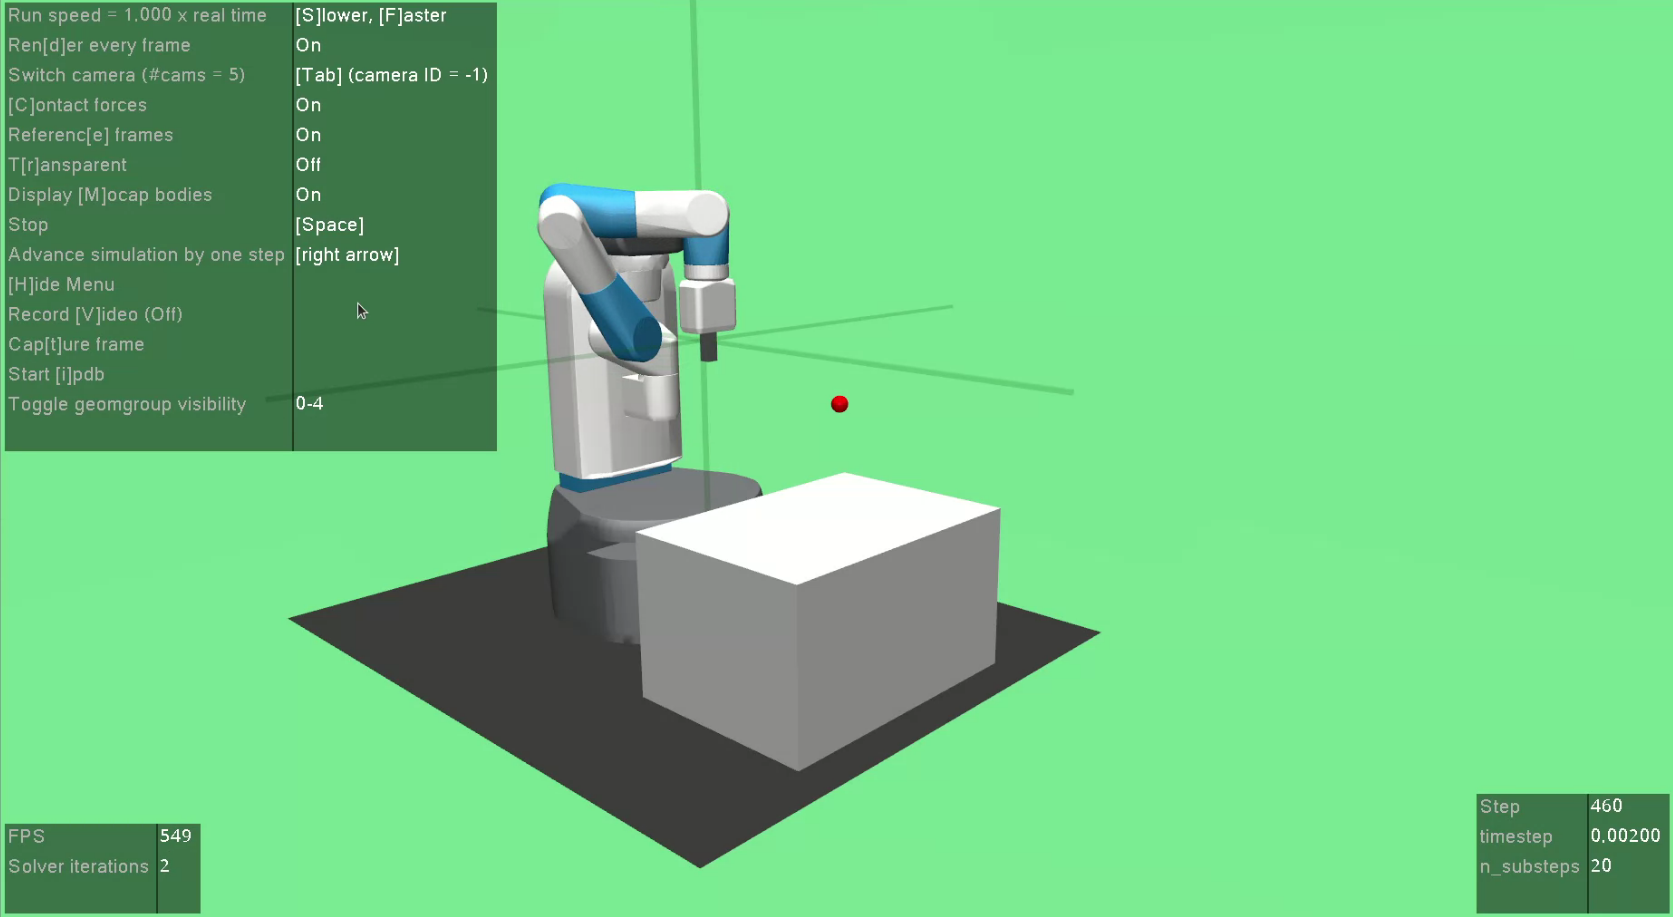
\includegraphics[width=0.8\textwidth]{fetchreach-v1.png}
        \caption{FetchReach-v1环境的截图}
        \label{fetchreach-v1}
    \end{figure}
其中有一个机械臂被放在一张桌子前。
在每个片段刚开始时,这个机械臂的状态都会被重置,而一个红点则会随机地出现在桌子上方的某处。
机械臂智能体需要在片段的限制时间内使自己的末端执行器到达这个红点附近来完成任务并获得奖励。
在片段的每一个时间步中,都会有观测值提供给此机械臂智能体。
观测值包括指示关节状态、末端执行器位置坐标信息作为已完成的目标,和红点的位置坐标信息作为期望目标。
指示关节状态的观测值$o\in \mathbb R^{10}$是一个10维的向量,而末端执行器的坐标$g^a \in \mathbb R^3$和红点的位置坐标$g^d\in\mathbb R^3$都是3维的向量。
因此提供给机械臂智能体的状态向量是一个16维的向量$s=(o, g^a, g^d)\in \mathbb R^{16}$。
如果末端执行器和红点之间的距离小于一个阈值,一个值为0.0的奖励会被提供给机械臂智能体,否则一个值为-1.0的奖励会被提供给它。
机械臂可以采取的动作是一个4维的取值在-1到1之间的向量,即$a\in[-1,1]^4$。

\section{Pyrobolearn和Pybullet}

\section{环境参数}
?
\section{系统设计}

系统由策略对象和奖励函数构成

% Local Variables:
% TeX-master: "../main"
% TeX-engine: xetex
% End:
